\documentclass[11pt,a4paper]{article}
\usepackage[margin=2.5cm]{geometry}
\usepackage{amsmath,amssymb}
\usepackage{booktabs,tabularx}
\usepackage{enumitem}
\usepackage{graphicx}
\usepackage{float}
\usepackage{xcolor}
\usepackage[colorlinks=true,linkcolor=blue!50!black]{hyperref}

\definecolor{boxbg}{HTML}{EEF3F8}
\definecolor{askbg}{HTML}{FFF1E0}
\newcommand{\idea}[1]{\par\smallskip\noindent\colorbox{boxbg}{\parbox{\dimexpr\linewidth-2\fboxsep}{\textbf{Recommendation.} #1}}\par\smallskip}
\definecolor{okbg}{HTML}{E6F4E7}
\newcommand{\agreed}[1]{\par\smallskip\noindent\colorbox{okbg}{\parbox{\dimexpr\linewidth-2\fboxsep}{\textbf{Agreed.} #1}}\par\smallskip}
\newcommand{\ask}[1]{\par\smallskip\noindent\colorbox{askbg}{\parbox{\dimexpr\linewidth-2\fboxsep}{\textbf{Your decision.} #1}}\par\smallskip}
\newcolumntype{Y}{>{\raggedright\arraybackslash}X}

\title{Proposal\\[2pt]\large Changes to ``How a run is scored'' (\texttt{sec:pf:measures})}
\author{For review before anything is applied}
\date{Version 2, 5 October 2026}

\begin{document}
\sloppy
\maketitle

\noindent This document collects every change proposed for the scoring
section of \texttt{Chapters/2.Introduction.tex}, so they can be reviewed
together before any of them is applied.

\paragraph{Current state.} The readability rewrite from earlier in this
session is in the working tree of \texttt{thesis/}. It is uncommitted and
changes only wording and order, not the model. Nothing else in this
document has been applied. The two figures shown here are drafts, saved
only in \texttt{scoring\_proposal/} at the workspace root and not in
\texttt{thesis/Images/}.

\paragraph{What changed in version 2.} Your answers are worked in. The
congestion part now follows your proposal and has no options left.
Robustness (C) and unfinished tasks (D) are explained with worked
examples, since you asked for more on both. Green boxes mark what is
agreed, and orange boxes mark what is still open.

\begin{center}
\begin{tabular}{lll}
  \toprule
  Item & Where & Status \\
  \midrule
  Fixes P1 to P11 that need no model decision & Section~\ref{sec:check} & please confirm \\
  A. What counts as even traffic & Section~\ref{sec:entropy} & open \\
  B. Congestion as the mean of $\delta_i(t)$ & Section~\ref{sec:congestion} & your proposal, please confirm \\
  C. Robustness & Section~\ref{sec:robust} & open, explained further \\
  D. Blocked time of unfinished tasks & Section~\ref{sec:unfinished} & open, explained further \\
  E. Keep ``movement cost'', add one clause & Section~\ref{sec:name} & agreed (E1) \\
  New structure of the section & Section~\ref{sec:structure} & agreed \\
  New concentration figure & Section~\ref{sec:figs} & agreed \\
  Timeline figure & Section~\ref{sec:figs} & agreed, one point to confirm \\
  \bottomrule
\end{tabular}
\end{center}

\tableofcontents

%----------------------------------------------------------------
\section{Check against the rest of the thesis}
\label{sec:check}

The section was compared with the Project Description (independent and
dependent variables, research questions), the task lifecycle, the
controller and congestion subsections, the scope subsection, the notation
table, and the Method chapter (reward, conflict resolution, instrumentation,
computational cost).

\subsection{What already matches}

\begin{itemize}[nosep]
  \item The seven dependent variables of the Project Description
    (service time, throughput, movement cost, waiting, concentration,
    backlog, runtime) are the seven quantities the section defines.
  \item The factors in \texttt{eq:rqformal} (window, congestion
    sensitivity, load $m$ and $\lambda_{\mathrm{task}}$, conditional
    communication) are the independent variables of the Project
    Description.
  \item $\tau_1$ in the toy table (released $5$, assigned $9$, finished
    $14$) matches the task example of \texttt{fig:taskroute} and
    \texttt{eq:lifecycle}.
  \item $\omega_j(t)$ comes from the override flag of the resolution
    operator, used the same way in the reward and in the instrumentation
    section.
  \item The notation table entries for $\Lambda_T$, $\bar\zeta_T$,
    $\mu_T$, $H_T$, $C_T$, $B_T$, $\omega_j$, $W_T$, $\kappa$ and the
    weights $q_\bullet$ agree with the section.
\end{itemize}

\subsection{What does not match}

\noindent The problems are numbered P1 to P11, so they are not confused with the options of the decisions below.


\noindent\begin{tabularx}{\linewidth}{@{}lYY@{}}
  \toprule
  & Mismatch & Proposed fix \\
  \midrule
  P1 & $\mu_T(e)$ is counted ``over the evaluation window''. Everywhere
       else ``window'' means what a controller may condition on
       (\texttt{tab:information}). The notation table repeats the phrase.
     & Say ``over the horizon $T$'' in the section and in
       \texttt{2.Notation.tex}. \\
  P2 & The section says how $\kappa(t)$ is measured ``is left to the
       implementation''. \texttt{sec:impl:cost} already fixes it:
       assignment and routing logged separately, same hardware, training
       and inference reported apart.
     & Point to \texttt{sec:impl:cost} and state that $\kappa(t)$ is the
       sum of the assignment and routing times. \\
  P3 & \texttt{eq:throughput} writes out
       $t_j^{\mathrm{finish}} - t_j^{\mathrm{released}}$, although
       $\zeta_j$ is already defined in \texttt{eq:servicetime}.
     & Write $\zeta_j$ and cite \texttt{eq:servicetime}. \\
  P4 & The text says ``congestion and concentration are reported as
       separate outcomes'' and the main RQ names congestion, but no
       congestion outcome is defined.
     & Decision~B, Section~\ref{sec:congestion}. \\
  P5 & The main RQ names ``robustness''. Nothing in the section measures
       it.
     & Decision~C, Section~\ref{sec:robust}. \\
  P6 & The Project Description calls $W_T$ ``waiting caused by
       contention''. $W_T$ also counts steps where the agent chose to
       wait with nobody in the way.
     & Change the Project Description to ``time blocked after
       assignment''. \\
  P7 & $W_T$ sums only over completed tasks. An agent stuck until the end
       never completes, so its blocked time never counts, and a deadlocked
       run can show a low $W_T$.
     & Decision~D, Section~\ref{sec:unfinished}. \\
  P8 & ``Movement cost'' $\bar c_T$ sums $\hat c$, which includes the
       waiting cost $c_{\mathrm{wait}}$ (\texttt{eq:onestepcost}).
     & Decision~E, Section~\ref{sec:name}. \\
  P9 & $\mathcal{J}$ takes expectations $\mathbb{E}[\cdot]$ without saying
       over what. The Method seeds the order stream, the policy and the
       environment separately.
     & One sentence saying the expectation is over the order stream and
       the random seeds, estimated by the mean over evaluation seeds. \\
  P10 & The constraints paragraph (\texttt{[G9]}) explains four of the
       five constraints in \texttt{eq:decisionproblem}.
       \texttt{eq:transition} is never mentioned, although the action
       space enforces it for every $\pi$ as well.
     & Add \texttt{eq:transition} to the group that holds by
       construction. \\
  P11 & The instrumentation section lists the logging of $H_T$,
       $\zeta_j$, $W_T$ and $B_T$, but not of $\bar c_T$.
     & One clause in \texttt{sec:impl:logging}. \\
  \bottomrule
\end{tabularx}

\medskip
\noindent Outside this section and not proposed for change now, the
Background chapter (\texttt{3.Background.tex}, around line 343) still
says ``information regimes''.

%----------------------------------------------------------------
\section{Decision A. What counts as ``even'' traffic}
\label{sec:entropy}

\subsection{Your question: how does the measure know it is a corridor?}

It does not know. The measure never looks at geometry. It only sees how
many times each edge was traversed. In this warehouse there is no open
space either. Every vertex is a position in an aisle and every edge is a
piece of aisle, so a ``corridor'' is simply a chain of edges, like the
eight edges from $a_4$ to D1 in Figure~\ref{fig:concdraft}.

The real question is what ``even'' is compared against. The current
definition divides by $\log|E^{+}_T|$, the number of edges that were used.
So it asks whether traffic is even among the edges the agents happened to
use. If all agents drive only along those eight edges, and evenly along
them, the answer is yes, and the run gets $H_T = 1$ and $C_T = 0$. That is
the score for perfectly spread traffic, although the whole fleet is in one
aisle. The bottom panel of Figure~\ref{fig:concdraft} shows this case.

\begin{figure}[H]
  \centering
  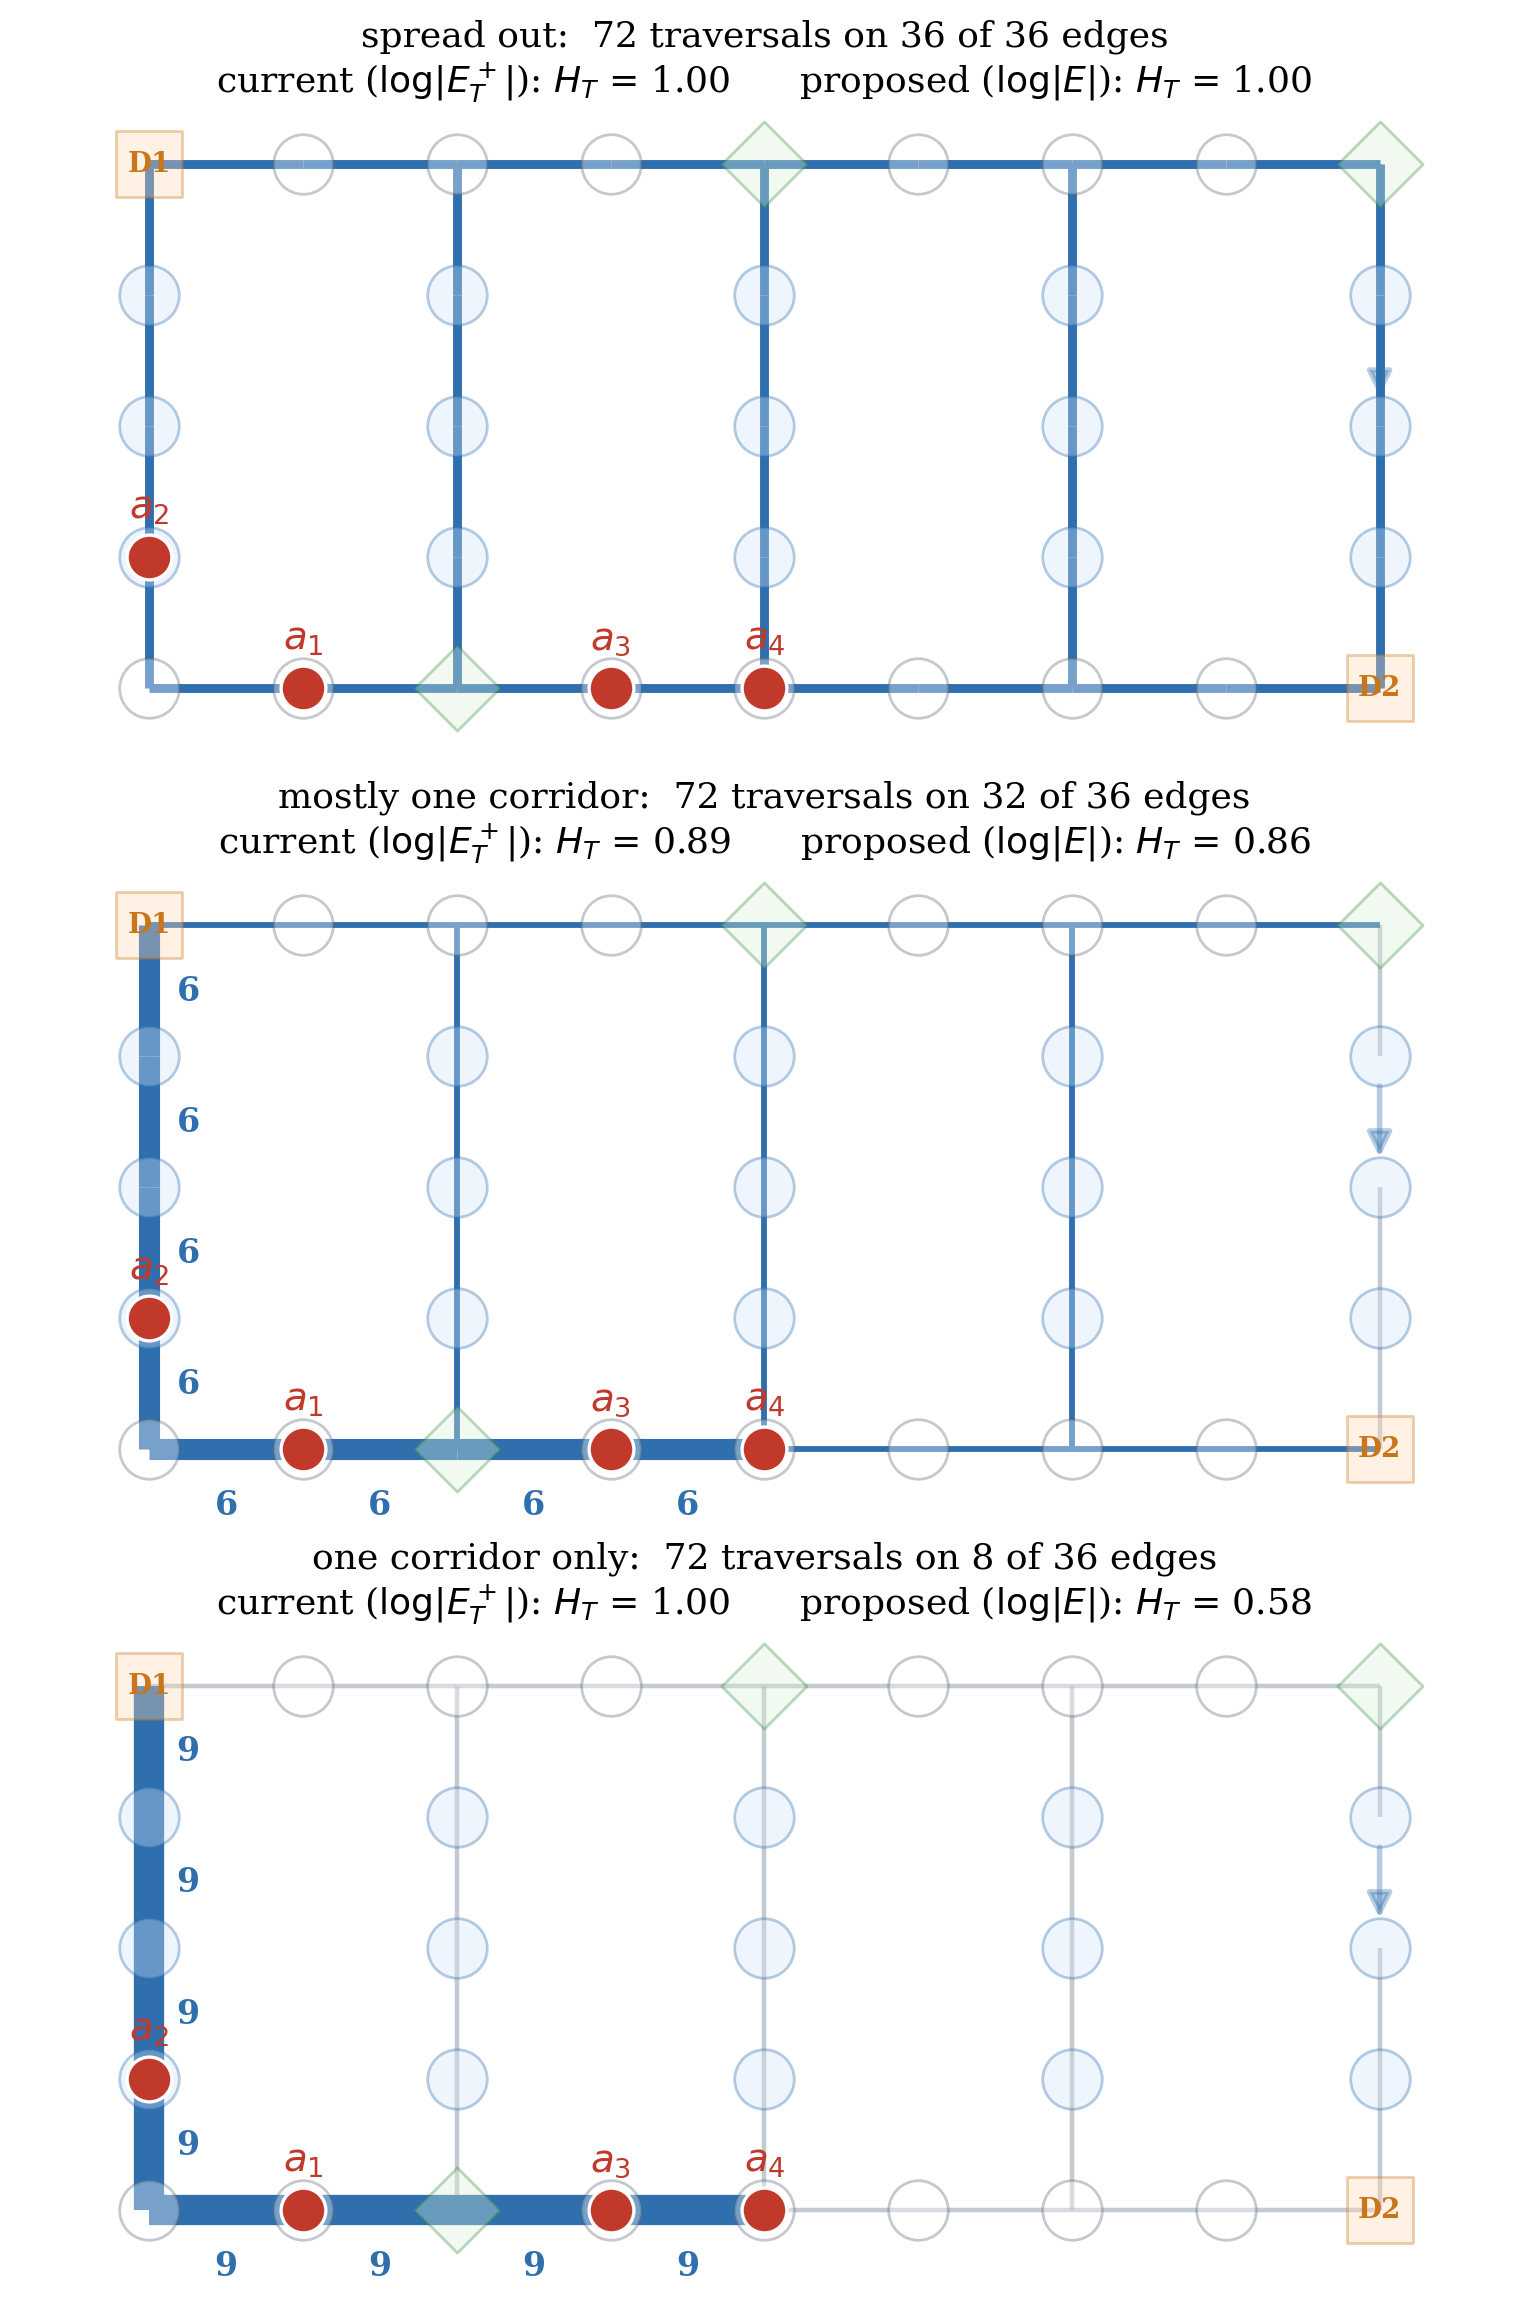
\includegraphics[width=0.78\linewidth]{concentration_draft.png}
  \caption{Draft of the new concentration figure, on the warehouse and agents of
  \texttt{observation.png}. Each panel has 72 traversals. The numbers are
  edge counts, and both normalisations are shown for comparison.}
  \label{fig:concdraft}
\end{figure}

\subsection{Options}

\begin{description}[leftmargin=1.5em]
  \item[A1. Divide by $\log|E|$, every edge in the graph.] ``Even'' then
    means even over the whole warehouse. One corridor only gives
    $H_T = 0.58$. The cost is that $H_T = 1$ is out of reach in practice,
    because some edges are never needed. That does not harm the study.
    The graph is the same in every condition, so the constant is the same
    for every run, and a comparison of $F_{\mathrm{fix}}$ with an adaptive
    $F$ stays fair. It also removes the stated limit that runs using
    different numbers of edges are not comparable.
  \item[A2. Keep $\log|E^{+}_T|$.] State the corridor case as a limit.
    $C_T$ then misses exactly the failure the RQ asks about, which is
    feedback piling traffic onto a few aisles.
  \item[A3. Report a simpler share as well.] The share of all
    traversals carried by the busiest 10\% of edges (4 of 36). This gives
    11\%, 33\% and 50\% for the three panels. A reader understands it at
    once, but it is not smooth enough to weight in $\mathcal{J}$.
\end{description}

\idea{A1 for $C_T$ in $\mathcal{J}$. Optionally add A3 as a reported
quantity, not weighted. A1 is a model change, logged as a new
\texttt{[Axx]} tag with a \texttt{GAPS.md} entry.}

\ask{Still open. A1, A2, or A1 with A3? The concentration figure is agreed either way. Only its numbers and the number of panels depend on this choice.}

%----------------------------------------------------------------
\section{Decision B. Measuring congestion with the congestion feature}
\label{sec:congestion}

\subsection{What you proposed}

Measure congestion with the same per-agent crowding reading that the
controllers already use, $\delta_i(t)$ (\texttt{eq:congestion}), the
fraction of an agent's field of view occupied by other agents. Version 1
offered this as option B2 next to the alternative of not measuring
crowding at all. You chose it, so the options are gone, and the version 1
subsection with the options is not needed any more.

\subsection{How it becomes a score}

$\delta_i(t)$ is one number per agent and per timestep. A run needs one
number in total, so the readings are averaged over every agent and every
timestep of the horizon,
\[
  \bar\delta_T = \frac{1}{mT}\sum_{t=0}^{T-1}\sum_{i=1}^{m}\delta_i(t) .
\]
For example, at $t = 11$ in \texttt{observation.png}, agent $a_1$ has
$\delta_1 = 2/5 = 0.4$. If the four agents read $0.4$, $0.2$, $0.4$ and
$0.2$ at every timestep, the run gets $\bar\delta_T = 0.3$, meaning that on
average 30\% of the space around an agent was taken.

The reading is defined the same way for every agent and every
architecture (\texttt{fig:congestion}). So $\bar\delta_T$ compares the
three controllers on equal terms, which is the reason the feature was
defined that way in the first place.

\subsection{How this relates to CRAMP}

CRAMP (Pham et al.\ 2024, arXiv 2309.10275, the paper behind the crowding feature) computes the same kind of density for each agent,
the number of agents in its field of view divided by the free space there.
It uses the density only inside its reward. An agent is penalised for
moving into an area whose density is above a threshold and rewarded for
moving out of one. CRAMP does not report the density as a result. Its
results are success rate, makespan, total moves and collision count
(Section~V-B of the paper).

So the thesis would use the CRAMP-style per-agent density in two places,
as the input that congestion-sensitive routing reacts to, which it
already does, and averaged into $\bar\delta_T$ as a reported outcome,
which is new. A CRAMP-style count of how often an agent stands in a
crowded area would need a threshold value that the thesis does not fix,
so the plain average is the simpler choice.

\subsection{Why $W_T$ stays as well}

$\bar\delta_T$ says how crowded it was. $W_T$ says how much time the
crowding cost. Agents moving in a tight convoy that never stops have a
high $\bar\delta_T$ and a $W_T$ of zero. The study needs both readings to
answer RQ3. When congestion sensitivity is switched on, $\bar\delta_T$
shows whether crowding went down, and $W_T$ shows whether that saved any
time.

$\bar\delta_T$ is reported and not weighted in $\mathcal{J}$. Its cost
already enters $\mathcal{J}$ through $W_T$, so weighting both would count
one effect twice.

\subsection{What changes in the thesis}

\begin{itemize}[nosep]
  \item One short paragraph and the formula for $\bar\delta_T$ in the
    waiting group of the scoring section. It points to
    \texttt{fig:congestion}, so no new picture is needed.
  \item The sentence ``congestion and concentration are reported as
    separate outcomes'' then names $\bar\delta_T$ and $W_T$.
  \item A row in the summary table (not in $\mathcal{J}$), a row in the
    notation table, an \texttt{[Axx]} tag and a \texttt{GAPS.md} entry.
  \item ``Crowding'' is added to the dependent variables in the Project
    Description.
\end{itemize}

\ask{Confirm that $\bar\delta_T$ is added this way, reported and not
weighted in $\mathcal{J}$.}

%----------------------------------------------------------------
\section{Decision C. What ``robustness'' means}
\label{sec:robust}

\subsection{The problem}

The main research question asks how coupling affects ``efficiency,
congestion, traffic concentration, and robustness''. Each of the first
three has its own quantity in the scoring section. Robustness has none,
and the thesis never says what it means by it.

\subsection{What robustness would mean here}

A gain is robust when it does not depend on luck or on one particular
setting. Two things can break a gain in this study. One is the random
seed, which decides the order stream and the training run. The other is
the load, the number of agents and how fast tasks arrive. The worked
example below shows the gain of adaptive storage over fixed storage,
$\mathcal{J}(F_{\mathrm{fix}},\pi) - \mathcal{J}(F,\pi)$ as a percentage,
over five seeds at two loads. The numbers are invented for illustration.

\begin{center}
\begin{tabular}{lccccccc}
  \toprule
  Load & seed 1 & seed 2 & seed 3 & seed 4 & seed 5 & mean & seeds where $F$ wins \\
  \midrule
  $m = 4$  & $+12$ & $+10$ & $+11$ & $+9$ & $+13$ & $+11$ & 5 of 5 \\
  $m = 12$ & $+25$ & $+30$ & $-5$ & $+28$ & $-8$ & $+14$ & 3 of 5 \\
  \bottomrule
\end{tabular}
\end{center}

\noindent At $m = 12$ the mean gain is larger, but in two of five seeds
adaptive storage is worse than fixed storage. The gain at $m = 4$ is
smaller and robust. The gain at $m = 12$ is larger and not robust. A
report of the means alone would rank them the wrong way round.

\subsection{The proposal}

No new formula. The scoring section gets two sentences that say
robustness is read from numbers the study already produces:
\begin{itemize}[nosep]
  \item the spread of each quantity across seeds, as the smallest and
    largest value, or as the number of seeds in which adaptive storage
    wins, as in the table above
  \item whether the gain keeps its sign as the load grows (RQ4), and
    whether the backlog $B_T$ stays bounded at high load
\end{itemize}
This matches \texttt{eq:rqformal}, which already asks for a margin
``exceeding seed variance''. The proposal gives that phrase the name the
RQ uses.

The alternative is to remove ``robustness'' from the main RQ. That is
simpler, but it drops a property the thesis does test.

\ask{C1, define robustness in two sentences as above, or C2, remove the
word from the RQ?}

%----------------------------------------------------------------
\section{Decision D. Blocked time of tasks that never finish}
\label{sec:unfinished}

\subsection{The problem with a worked example}

$W_T$ averages the blocked time over completed tasks only. Take the three
tasks of the timeline figure and add a fourth, $\tau_4$. It is released at
$11$, assigned at $12$, gets stuck at $14$, and is still stuck when the
run ends at $T = 20$ (Figure~\ref{fig:stuck}).

\begin{figure}[H]
  \centering
  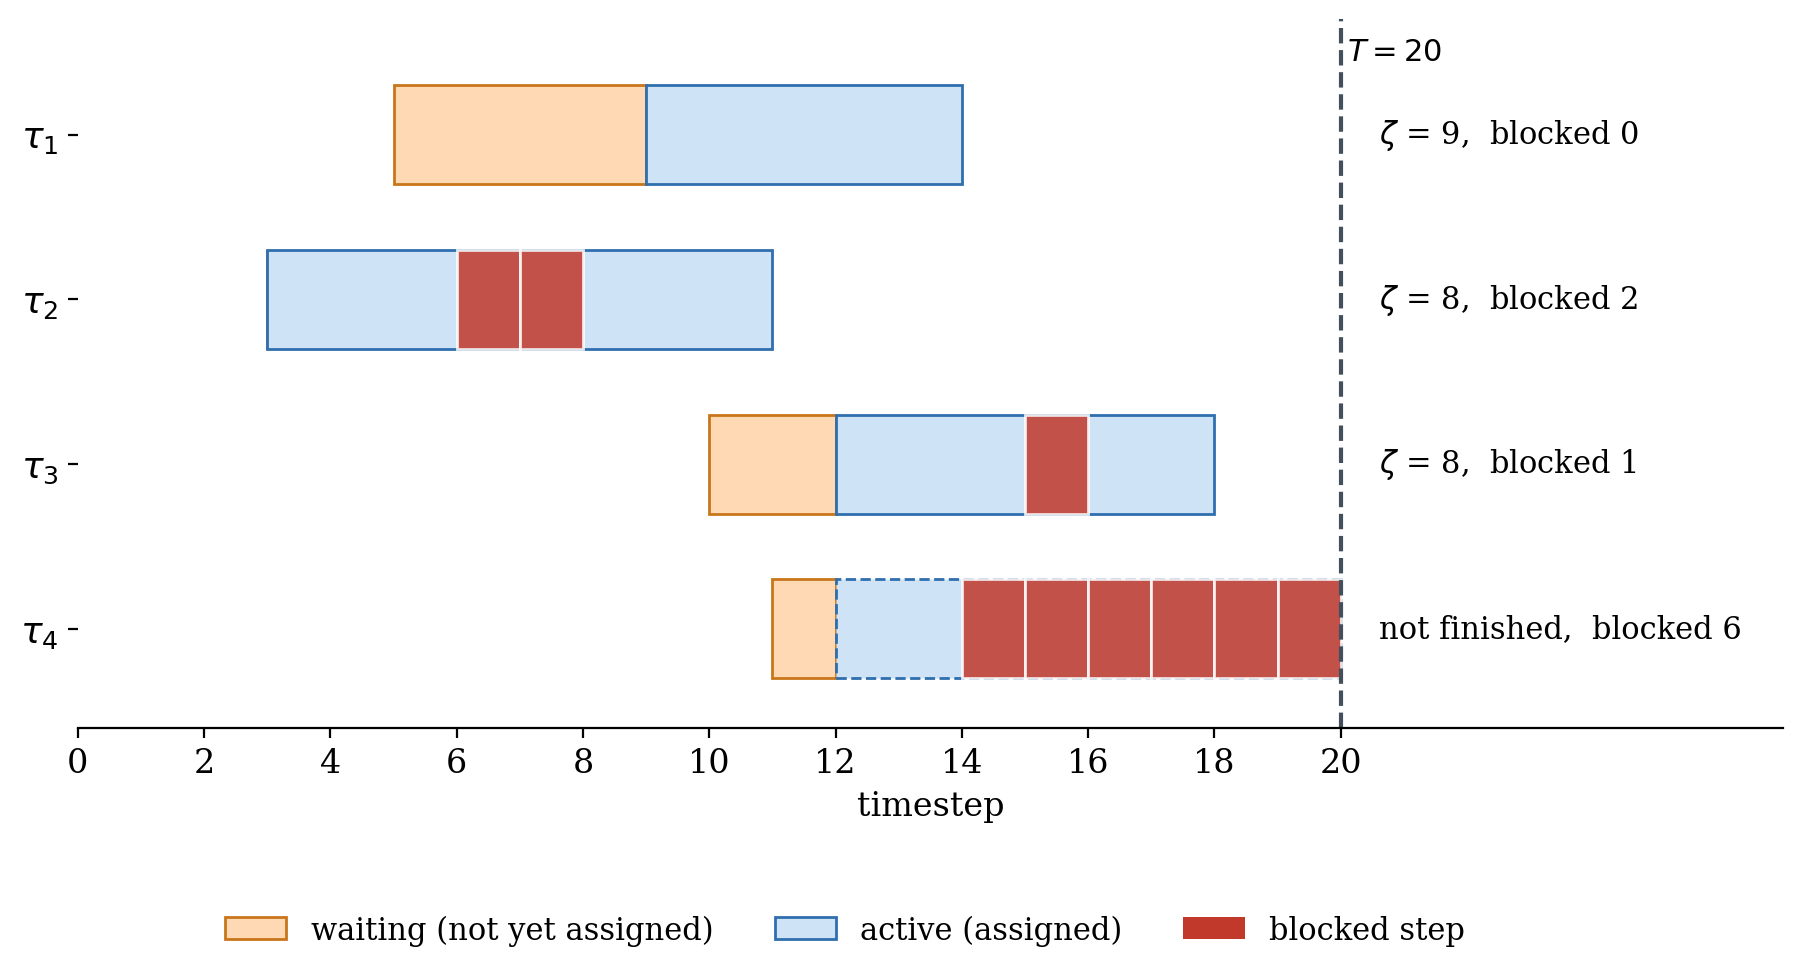
\includegraphics[width=0.85\linewidth]{timeline_stuck_draft.png}
  \caption{The timeline example with a fourth task $\tau_4$ that is stuck from
  $t = 14$ and never finishes.}
  \label{fig:stuck}
\end{figure}

\noindent The two options give these numbers for this run.

\begin{center}
\begin{tabular}{lcc}
  \toprule
  & D1, completed tasks only & D2, every assigned task \\
  \midrule
  $W_T$       & $(0+2+1)/3 = 1$ & $(0+2+1+6)/4 = 2.25$ \\
  $\bar\zeta_T$ & $8.33$ & $8.33$ \\
  $B_T$       & $1$ & $1$ \\
  age of $\tau_4$ at $T$ & $9$ & $9$ \\
  \bottomrule
\end{tabular}
\end{center}

\noindent Under D1, $W_T$ is $1$ with or without the stuck task, so $W_T$
alone cannot see it. The run is still not hidden. $\tau_4$ adds one to the
backlog $B_T$, which is weighted in $\mathcal{J}$, and its age of $9$
timesteps is reported with the unfinished tasks.

\subsection{The two options}

\begin{description}[leftmargin=1.5em]
  \item[D1. Keep $W_T$ as it is, and say why.] Every per-task average in
    the section (service time, movement cost, blocked time) is taken over
    the same completed tasks, so they can be compared directly. Unfinished
    work is the job of one quantity, the backlog. This needs one sentence
    in the thesis and no model change.
  \item[D2. Count every assigned task.] $W_T$ also sees the stuck task.
    The cost is that $W_T$ is then averaged over a different set of tasks
    than $\bar\zeta_T$ and $\bar c_T$, and a task that is stuck counts
    twice in $\mathcal{J}$, once through $W_T$ and once through $B_T$.
    This is a model change.
\end{description}

\idea{D1. It is the same rule service time already follows, since
$\bar\zeta_T$ also ignores $\tau_4$. The worked example shows that the
backlog catches the stuck task. D2 would mostly punish the same task a
second time.}

\ask{D1 or D2?}

%----------------------------------------------------------------
\section{Decision E. The name ``movement cost''}
\label{sec:name}

\agreed{E1. Keep the name and add one clause saying that standing still
costs $c_{\mathrm{wait}}$ per timestep, so $\bar c_T$ counts it too.}

%----------------------------------------------------------------
\section{New structure of the section}
\label{sec:structure}

\agreed{The structure below. The waiting group now also holds the crowding
measure $\bar\delta_T$ from Decision B.}

\noindent The reader first gets a plain overview, then one
group of quantities at a time under a \verb|\paragraph| heading. The
summary table moves to just after $\mathcal{J}$, where every symbol in it
has been met.

\begin{enumerate}[nosep]
  \item \textbf{Overview}, with no symbols. A run answers three questions:
    how much work was done, what it cost, and how evenly traffic spread.
    One criterion then combines them.
  \item \textbf{Completed work.} Throughput $\Lambda_T$ and mean service
    time $\bar\zeta_T$, with the timeline figure (Section~\ref{sec:figs}).
  \item \textbf{Cost of the work.} $\bar c_T$.
  \item \textbf{Unfinished work.} Backlog $B_T$.
  \item \textbf{Waiting and crowding.} $W_T$ on the same timeline figure,
    how it differs from $\hat w_t(e)$, then $\bar\delta_T$ with a pointer
    to \texttt{fig:congestion}.
  \item \textbf{Traffic spread.} $H_T$ and $C_T$ with the new
    concentration figure, then its limits.
  \item \textbf{The criterion.} $\mathcal{J}$, why throughput is left out,
    then the summary table.
  \item \textbf{Runtime.} $\kappa_T$ and why it stays out of
    $\mathcal{J}$.
  \item \textbf{The decision problem.} \texttt{eq:decisionproblem}, the
    constraints, \texttt{eq:rqformal} and its factors, and robustness
    (Decision C).
\end{enumerate}

\noindent The per-task quantities (2 to 5) come before the per-edge ones
(6), so the timeline figure serves four measures in a row. The line
``Figure~12 shows the two extremes'' disappears as a sentence of its own.
The figure is referred to inside the paragraph that introduces $C_T$.

The proposed opening paragraph reads:

\begin{quote}\small
A run is judged by three questions. How much work did the agents
complete, what did that work cost, and how evenly did the traffic spread
over the warehouse while they did it? Each question is answered by one or
two numbers, defined below one group at a time. Five of them are then
combined into a single score for the run, and the others are reported
next to it.
\end{quote}

%----------------------------------------------------------------
\section{Figures}
\label{sec:figs}

\subsection{Concentration figure (replaces \texttt{concentration.png})}

\agreed{The new figure replaces \texttt{concentration.png}.}

Figure~\ref{fig:concdraft} is the draft. It is built on the same base as
\texttt{observation.png}: the dimmed warehouse with vertex roles, D1 and
D2, and agents $a_1$ to $a_4$ at the same positions ($m = 4$). Edge width
and the printed numbers are traversal counts. The thesis version would
keep two panels, or three under A1, since the third panel is the case that
motivates A1. The two normalisations are printed only in this draft.

The text example of three edges used $8$, $1$ and $1$ times would be
replaced by the figure's numbers: 72 traversals, the eight edges from
$a_4$ to D1 used six times each, and the D2 aisle unused.

\subsection{Timeline figure (new, replaces \texttt{tab:throughputexample})}

\begin{figure}[H]
  \centering
  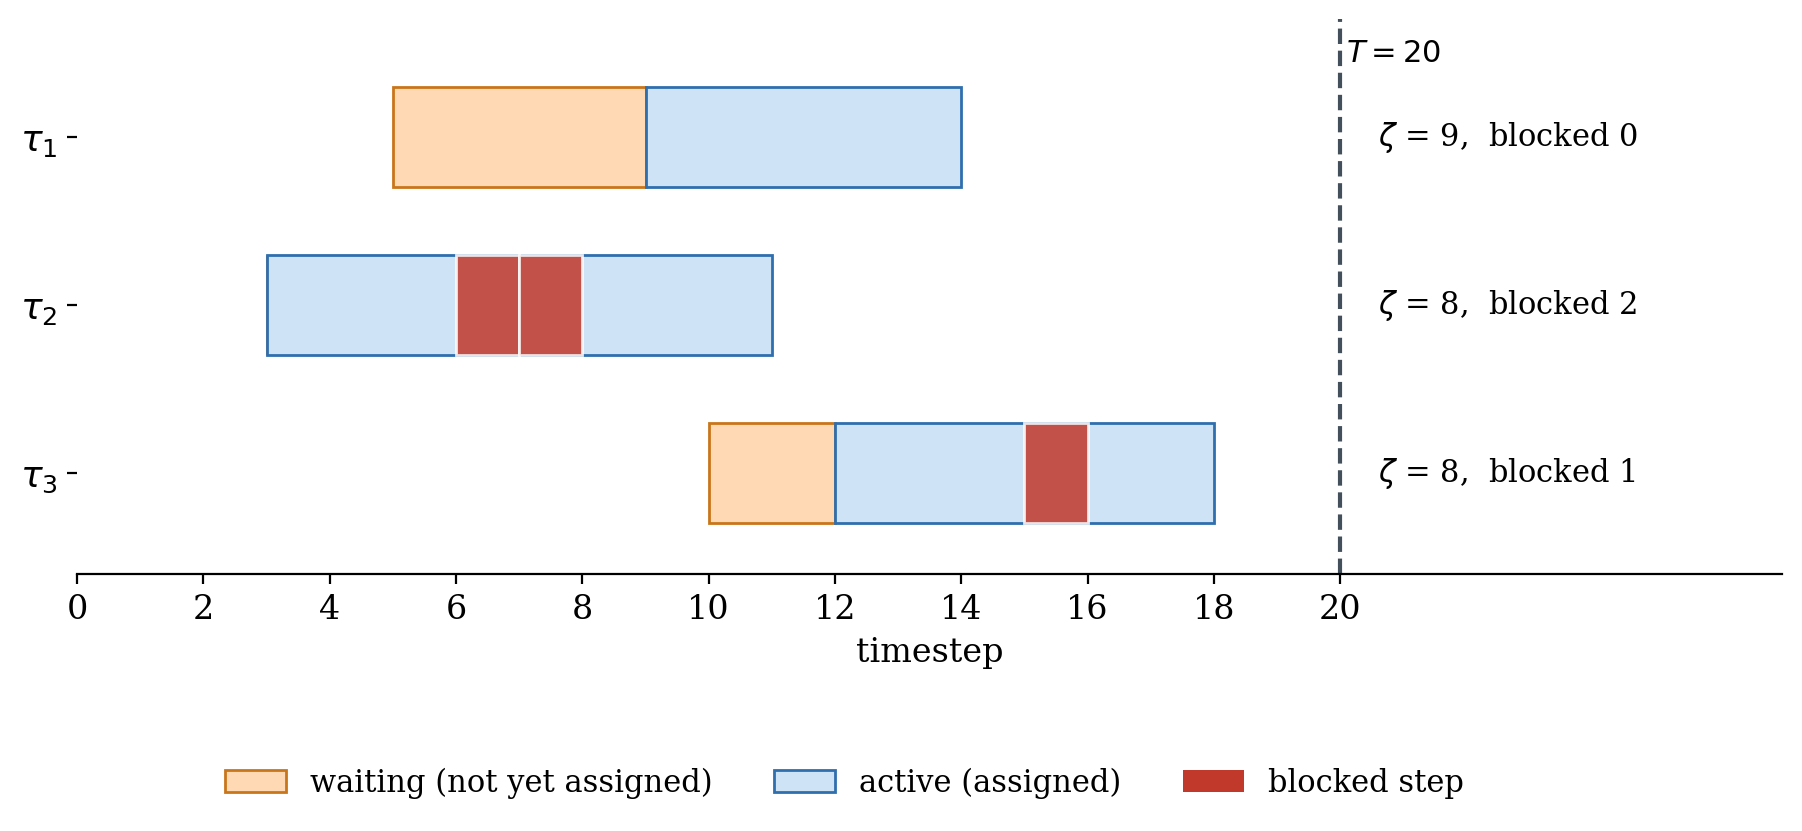
\includegraphics[width=0.85\linewidth]{timeline_draft.png}
  \caption{Draft timeline of the three tasks of the toy table, with blocked
  steps. It gives $\bar\zeta_T \approx 8.33$, $\Lambda_T = 0.15$ and
  $W_T = (0+2+1)/3 = 1$.}
  \label{fig:timeline}
\end{figure}

You asked for the blocked steps to be added to \texttt{lifecycle.png}.
That does not work without contradicting the task example. In
\texttt{fig:taskroute}, $a_2$ moves from its start at $t=9$ to $A$ at
$t=11$ and to D1 at $t=14$, one edge per timestep. It is never blocked,
so $\tau_1$ contributes $0$ to $W_T$.

The draft instead draws the three tasks of the toy table on one time axis
and gives $\tau_2$ and $\tau_3$ a few blocked steps. One figure then shows
service time, throughput and blocked time at once. It can replace the toy
table, whose numbers it contains. \texttt{lifecycle.png} stays as it is.

\agreed{The timeline figure is added.}

\ask{You wrote ``keep 6.2''. I read that as adding the timeline figure
and dropping the toy table, since the figure holds its numbers. If you
meant that the toy table should stay next to the figure, say so.}

\subsection{Crowding figure}

No new figure is needed. The crowding measure $\bar\delta_T$ points to
\texttt{fig:congestion}, which already shows how $\delta_i(t)$ is read for
each agent.

%----------------------------------------------------------------
\section{What will be applied once you decide}

\begin{enumerate}[nosep]
  \item Restructure the section as in Section~\ref{sec:structure}.
  \item Fixes P1, P2, P3, P6, P9, P10 and P11, which need no model
    decision.
  \item Decisions A to E as chosen (B and E as above), each model change with an
    \texttt{[Axx]} tag, a \texttt{GAPS.md} entry and a notation table
    update.
  \item Add the figure scripts to \texttt{thesis-progress/scripts/images/},
    with outputs copied to both \texttt{Images/} folders.
  \item Build the thesis, check \texttt{git diff main.tex} for stray
    text, and commit only after you have read the result.
\end{enumerate}

\end{document}
